\documentclass[20pt,landscape,a4paper,footrule]{foils}
\usepackage{zencurity-slides}
\usepackage{pdf14}
%
% Penetration testing III - Wireless sikkerhed
% Mål:	Introduktion til penetrationstest af wireless netværk.

% Forudsætninger:	Der forventes kendskab til TCP/IP på brugerniveau.
% Beskrivelse:	Trådløse netværk er overalt og alle nye bærbare
% computere leveres som standard med trådløse netkort. Desværre er
% sikkerheden i de trådløse netværk ikke altid god nok og det giver
% anledning til bekymring.

% * Sikkerhedsteknologier i 802.11b - WEP, forkortes, men stadig relevant
% * Sikkerhedsteknologier i 802.11g - WPA, WPA2, WPS
% * wardriving med scannerprogrammer som Kismet og netstumbler
% * airodump og aircrack-ng
% * Packet injection med wireless værktøjer
% * Opsætning af trådløse netværk og forbindelse til andre netværk

% Der vil være demonstrationer af sårbarheder på alle foredragene - typisk med
% open source programmer, således at deltagerne kan afprøve de selvsamme demoer
% hjemme.

% Note: der tages udgangspunkt i open source og UNIX.



\begin{document}


%{Penetration testing II\\\normalsize webbaserede angreb}

\mytitlepage
{Penetration testing III\\ Wireless sikkerhed}

%\begin{alltt}
%\tiny
%\centerline{$Id: pentest-III-foredrag.tex,v 1.3 2008/03/05 13:06:36 hlk Exp $}
%\end{alltt}

\LogoOn


%\dagsplan

\slide{Formålet idag}
\vskip 2 cm

\hlkimage{5cm}{dont-panic.png}
\centerline{\color{titlecolor}\LARGE Don't Panic!}

\begin{list1}
\item At vise de sikkerhedsmæssige aspekter af trådløse netværk

\item At inspirere jer til at implementere trådløse netværk sikkert

\item At fortælle jer om nogle af mulighederne for sikring af de
  trådløse netværk
\end{list1}

\slide{Planen idag}

\hlkimage{10cm}{Shaking-hands_web.jpg}

\begin{list1}
\item Kl 17-21
\item Mindre foredrag mere snak
\item Mindre enetale, mere foredrag 2.0 med socialt medie, informationsdeling og interaktion
\end{list1}

\slide{Hacker - cracker}

{\bfseries Det korte svar - drop diskussionen}

%Det lidt længere svar:\\
Det havde oprindeligt en anden betydning, men medierne har taget
udtrykket til sig - og idag har det begge betydninger.

{\color{red}\hlkbig Idag er en hacker stadig en der bryder ind i systemer!}

ref. Spafford, Cheswick, Garfinkel, Stoll, ...
- alle kendte navne indenfor sikkerhed

Hvis man vil vide mere kan man starte med:
\begin{list2}
\item \emph{Cuckoo's Egg: Tracking a Spy Through the Maze of Computer
 Espionage},  Clifford Stoll
\item \emph{Hackers: Heroes of the Computer Revolution},
Steven Levy
\item \emph{Practical Unix and Internet Security},
Simson Garfinkel, Gene Spafford, Alan Schwartz
\end{list2}

\slide{Definition af hacking, oprindeligt}

\begin{quote}
Eric Raymond, der vedligeholder en ordbog over computer-slang (The Jargon File) har blandt andet følgende forklaringer på ordet hacker:
\begin{list2}
\item En person, der nyder at undersøge detaljer i programmerbare systemer og hvordan man udvider deres anvendelsesmuligheder i modsætning til de fleste brugere, der bare lærer det mest nødvendige
\item En som programmerer lidenskabligt (eller enddog fanatisk) eller en der foretrækker at programmere fremfor at teoretiserer om det
\item En ekspert i et bestemt program eller en der ofter arbejder med eller på det; som i "en Unixhacker".
\end{list2}
\end{quote}

\begin{list1}
\item Source: Peter Makholm, \link{http://hacking.dk}
\item Benyttes stadig i visse sammenhænge se \link{http://labitat.dk}
\end{list1}


\slide{Aftale om test af netværk}

{\bfseries Straffelovens paragraf 263 Stk. 2. Med bøde eller fængsel
  indtil 6 måneder
straffes den, som uberettiget skaffer sig adgang til en andens
oplysninger eller programmer, der er bestemt til at bruges i et anlæg
til elektronisk databehandling.}

Hacking kan betyde:
\begin{list2}
\item At man skal betale erstatning til personer eller virksomheder
\item At man får konfiskeret sit udstyr af politiet
\item At man, hvis man er over 15 år og bliver dømt for hacking, kan
  få en bøde - eller fængselsstraf i alvorlige tilfælde
\item At man, hvis man er over 15 år og bliver dømt for hacking, får
en plettet straffeattest. Det kan give problemer, hvis man skal finde
et job eller hvis man skal rejse til visse lande, fx USA og
Australien
\item Frit efter: \link{http://www.stophacking.dk} lavet af Det
  Kriminalpræventive Råd
\item Frygten for terror har forstærket ovenstående - så lad være!
\end{list2}

\slide{Er trådløst interessant?}

\centerline{\color{titlecolor}\LARGE\bf wireless 802.11}
\hlkimage{3cm}{12065572121317625675no_hope_Wireless_access_point.png}


\begin{list1}
\item Wireless er lækkert
\item Wireless er nemt
\item Wireless er praktisk
\item Alle nye bærbare leveres med wireless kort
\item Jeg bruger selv næsten udelukkende wireless på min laptop
\end{list1}

\slide{Hacking er magi}

\hlkimage{7cm}{wizard_in_blue_hat.png}

\vskip 1 cm

\centerline{Hacking ligner indimellem  magi}


\slide{Hacking er ikke magi}

\hlkimage{17cm}{ninjas.png}

\vskip 1 cm
\centerline{Hacking kræver blot lidt ninja-træning}


\slide{Hacking eksempel - det er ikke magi}

\hlkimage{20cm}{ethernet-frame-1.pdf}

\begin{list1}
\item MAC filtrering på trådløse netværk - Alle netkort har en MAC fra fabrikken
\item Mange trådløse Access Points kan filtrere MAC adresser
\item Kun kort som er på listen over godkendte adresser tillades adgang til netværket
\pause
\item Det virker dog ikke \smiley
\item De fleste netkort tillader at man overskriver denne adresse midlertidigt
%\item Derudover har der ofte været fejl i implementeringen af MAC filtrering
\end{list1}

\slide{Myten om MAC filtrering}

\begin{list1}
\item Eksemplet med MAC filtrering er en af de mange myter
\item Hvorfor sker det?
\begin{list2}
\item Marketing - producenterne sætter store mærkater på æskerne
\item Manglende indsigt - forbrugerne kender reelt ikke koncepterne
\item Hvad \emph{er} en MAC adresse egentlig
\item Relativt få har forudsætningerne for at gennemskue dårlig sikkerhed
\end{list2}
\item Løsninger?
\pause
\begin{list2}
\item Udbrede viden om usikre metoder til at sikre data og computere
\item Udbrede viden om sikre metoder til at sikre data og computere
\end{list2}
\end{list1}

\slide{MAC filtrering}

\hlkimage{15cm}{stupid-security.jpg}



\slide{Konsekvenserne}

\hlkimage{10cm}{images/wireless-daekning.pdf}

\begin{list2}
\item Værre end Internetangreb - anonymt
\item Kræver ikke fysisk adgang til lokationer
%\emph{spioneres imod}
\item Konsekvenserne ved sikkerhedsbrud er generelt større
\item Typisk får man direkte LAN eller Internet adgang!
\end{list2}


\slide{IEEE 802.11 Security fast forward }

\begin{quote}
{\bf In 2001}, a group from the University of California, Berkeley presented a paper describing weaknesses in the 802.11 Wired Equivalent Privacy (WEP) security mechanism defined in the original standard; they were followed by {\bf Fluhrer, Mantin, and Shamir's} paper titled "Weaknesses in the Key Scheduling Algorithm of RC4". Not long after, Adam Stubblefield and AT\&T publicly announced the first {\bf verification of the attack}. In the attack, they were able to intercept transmissions and gain unauthorized access to wireless networks.
\end{quote}
Source: \link{http://en.wikipedia.org/wiki/IEEE_802.11}

\slide{IEEE 802.11 Security fast forward }

\begin{quote}
The IEEE set up a dedicated task group to create a replacement security solution, {\bf 802.11i} (previously this work was handled as part of a broader 802.11e effort to enhance the MAC layer). The Wi-Fi Alliance announced an {\bf interim specification called Wi-Fi Protected Access (WPA)} based on a subset of the then current IEEE 802.11i draft. These started to appear in products in {\bf mid-2003}. {\bf IEEE 802.11i (also known as WPA2)} itself was ratified in {\bf June 2004}, and uses government strength encryption in the {\bf Advanced Encryption Standard AES,} instead of RC4, which was used in WEP. The modern recommended encryption for the home/consumer space is {\bf WPA2 (AES Pre-Shared Key) and for the Enterprise space is WPA2 along with a RADIUS authentication server} (or another type of authentication server) and a strong authentication method such as EAP-TLS.
\end{quote}
Source: \link{http://en.wikipedia.org/wiki/IEEE_802.11}

\slide{IEEE 802.11 Security fast forward }

\begin{quote}
In January 2005, the IEEE set up yet another task group "w" to protect management and broadcast frames, which previously were sent unsecured. Its standard was published in 2009.[24]

In {\bf December 2011}, a security flaw was revealed that affects wireless routers with the {\bf optional Wi-Fi Protected Setup (WPS)} feature. While WPS is not a part of 802.11, {\bf the flaw allows a remote attacker to recover the WPS PIN and, with it, the router's 802.11i password in a few hours}.
\end{quote}

\vskip 2cm
\centerline{WPS WTF?! - det er som om folk bevidst saboterer wireless sikkerhed!}
\vskip 2cm

Source: \link{http://en.wikipedia.org/wiki/IEEE_802.11}


\slide{Emneområder}


\begin{list1}
\item Introduktion - begreber og teknologierne
\item Basal konfiguration af trådløst IEEE802.11 - wardriving
\item Hacking af trådløse netværk - portscanning, exploits
\item Sikkerhedsteknologier i 802.11b - WEP, forkortes, men stadig relevant
\item Sikkerhedsteknologier i 802.11i - WPA, WPA2
\item airodump og aircrack-ng
\item Packet injection med wireless værktøjer
\item Infrastrukturændringer, segmentering og firewall konfiguration
\end{list1}

\vskip 1 cm

\centerline{\hlkbig Husk: trådløs sikkerhed er ikke kun kryptering}


\slide{Værktøjer}

\hlkimage{15cm}{kali-linux.png}

\begin{list1}
\item Alle bruger nogenlunde de samme værktøjer, måske forskellige
  mærker
\begin{list2}
\item Wirelessscanner - Kismet og BackTrack/Kali
\item Wireless Injection - typisk på Linux
\item ...
\item Aircrack-ng
\end{list2}
\item Kali \link{http://www.kali.org/}
\end{list1}



\slide{Konsulentens udstyr wireless}

\begin{list1}
\item Laptop or Netbook, I typically use USB wireless cards\\
{\bf NB: de indbyggede er ofte ringe - så check før køb ;-)}
\item Access Points - get a small selection for testing
\item Books and Internet:
\begin{list2}
\item \emph{Metasploit The Penetration Tester's Guide}
by David Kennedy, Jim O'Gorman, Devon Kearns, and Mati Aharoni
http://nostarch.com/metasploit
\item \emph{Hacking Exposed Wireless, Second Edition}
\item \emph{Gray Hat Hacking: The Ethical Hacker's Handbook}, 3rd Edition, Shon Harris et al, Osborne
\item \emph{Counter Hack Reloaded: A Step-by-Step Guide to Computer Attacks and Effective Defenses} (2nd Edition), Ed Skoudis, Prentice Hall PTR
\item Kali \link{http://www.kali.org/}
\item Packetstorm wireless tools
\link{http://packetstormsecurity.org/wireless/}
\item \emph{Beginner's Guide to Wireless Auditing}
David Maynor great story\\
\link{http://www.securityfocus.com/infocus/1877?ref=rss}
\end{list2}
\end{list1}

\slide{Pwnie express}

\hlkimage{13cm}{pwnie-express-pwnpad.png}

Source: \link{http://pwnieexpress.com/products/pwnpad}

Note: old picture, price is now \$1.095 and just an example\\
 - tablets are great for some wireless testing

\slide{Hackerværktøjer}
% måske til reference afsnit?

\begin{list1}
\item Der benyttes en del værktøjer:
\begin{list2}
\item Nmap, Nping - tester porte, godt til firewall admins \link{http://nmap.org}
\item Metasploit Framework gratis på \link{http://www.metasploit.com/}
\item Wireshark avanceret netværkssniffer - \link{http://http://www.wireshark.org/}

\item Kismet \link {http://www.kismetwireless.net/}
\item Kismac \link{http://kismac-ng.org/}

\item Aircrack-ng set of tools \link{http://www.aircrack-ng.org/}
\item Bruteforge \link{http://masterzorag.blogspot.com/}
\item Pyrit GPU cracker \link{http://code.google.com/p/pyrit/}
\item Reaver brute force WPS \link{https://code.google.com/p/reaver-wps/}
\end{list2}
\end{list1}

\slide{it's a Unix system, I know this}

\hlkimage{24cm}{twitter-unix-security.png}

\begin{list1}
\item Skal du igang med sikkerhed?
\item Installer et netværk, evt. bare en VMware, Virtualbox, Parallels, Xen, GNS3, ...
\item Brug Kali Linux, se evt. youtube videoer om programmerne\\
- det er en værktøjskasse du tager frem ikke en kult \smiley
\end{list1}

Quote fra Jurassic Park
\link{http://www.youtube.com/watch?v=dFUlAQZB9Ng}

\slide{Hvad skal der ske?}

\begin{list1}
\item Tænk som en hacker
\item Rekognoscering
\begin{list2}
\item ping sweep, port scan
\item OS detection - TCP/IP eller banner grab
\item Servicescan - rpcinfo, netbios, ...
\item telnet/netcat interaktion med services
\end{list2}
\item Udnyttelse/afprøvning: Nessus, nikto, exploit programs
\item Oprydning/hærdning vises måske ikke, men I bør i praksis:
\end{list1}

\vskip 1cm
\centerline{\hlkbig Vi går idag kun efter wireless}

\slide{Internet idag og trådløse netværk}

\hlkimage{14cm}{images/server-client.pdf}

\begin{list1}
\item Klienter og servere
\item Rødder i akademiske miljøer
\item Protokoller der er op til 20 år gamle
\item Meget lidt kryptering, mest på http til brug ved e-handel
\end{list1}

\slide{OSI og Internet modellerne}

\hlkimage{14cm,angle=90}{images/compare-osi-ip.pdf}

\slide{Trådløse teknologier IEEE802.11}

\begin{list1}
\item 802.11 er arbejdsgruppen under IEEE
\item De mest kendte standarder idag indenfor trådløse teknologier:
\begin{list2}
\item 802.11b 11Mbps versionen
\item 802.11g 54Mbps versionen
\item 802.11n endnu hurtigere
\item 802.11i Security enhancements
\end{list2}
\end{list1}

Sourcer:
\link{http://en.wikipedia.org/wiki/IEEE_802.11}\\
\link{http://grouper.ieee.org/groups/802/11/index.html}


\slide{802.11 modes og frekvenser}

\begin{list1}
\item Access point kører typisk i \emph{access point mode} også kaldet
  infrastructure mode - al trafik går via AP
\item Alternativt kan wireless kort oprette ad-hoc netværk - hvor
  trafikken går direkte mellem netkort
%\item Frekvenser op til kanal 11 og 12+13 i DK/EU
%\item Helst 2 kanaler spring for 802.11b AP der placeres indenfor rækkevidde
%\item Helst 4 kanaler spring for 802.11g AP der placeres indenfor rækkevidde
\end{list1}

\slide{Eksempel på netværk med flere AP'er}

\hlkimage{20cm}{images/wireless-multi-ap.pdf}

\slide{Eksempel på netværk med flere AP'er}

\hlkimage{20cm}{images/wireless-multi-ap-2.pdf}


\slide{Wireless Distribution System WDS}

\hlkimage{18cm}{images/wireless-multi-ap-wds.pdf}

\begin{list1}
\item Se også:
\link{http://en.wikipedia.org/wiki/Wireless_Distribution_System}
\end{list1}


%\slide{Infrastrukturændringer}
\slide{Typisk brug af 802.11 udstyr}

\begin{center}
\colorbox{white}{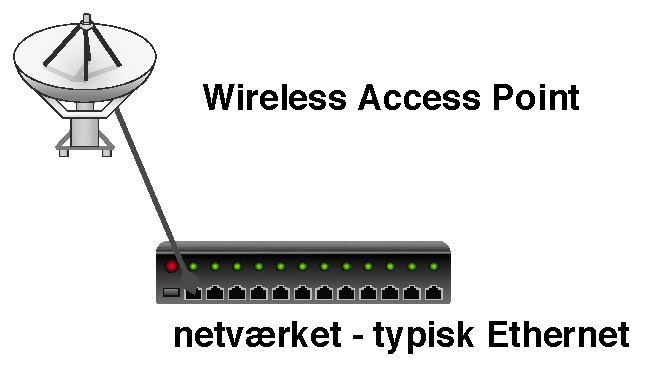
\includegraphics[width=20cm]{images/wlan-accesspoint-1.pdf}}
\end{center}

\centerline{\hlkbig et access point - forbindes til netværket}

\slide{Basal konfiguration}

\begin{list1}
\item Når man tager fat på udstyr til trådløse netværk opdager man:
\item SSID - nettet skal have et navn
\item frekvens / kanal - man skal vælge en kanal, eller udstyret
  vælger en automatisk
\item der er nogle forskellige metoder til sikkerhed
\end{list1}


\slide{Wireless networking sikkerhed i 802.11b}

\hlkimage{8cm}{images/wlan-accesspoint-1.pdf}

\begin{list1}
\item Sikkerheden er baseret på nogle få forudsætninger
  \begin{list2}
  \item SSID - netnavnet
  \item WEP \emph{kryptering} - Wired Equivalent Privacy
  \item måske MAC flitrering, kun bestemte kort må tilgå accesspoint
  \end{list2}
\item Til gengæld er disse forudsætninger ofte ikke tilstrækkelige ...
%\item Hvorfor hader du WEP?
  \begin{list2}
  \item WEP er måske \emph{ok} til visse små hjemmenetværk
  \item WEP er baseret på en DELT hemmelighed som alle stationer kender
  \item nøglen ændres sjældent, og det er svært at distribuere en ny
  \end{list2}

\end{list1}


\slide{Forudsætninger}

\begin{list1}
\item Til gengæld er disse forudsætninger ofte ikke tilstrækkelige ...
\item Hvad skal man beskytte?
\item Hvordan kan sikkerheden omgås?
\item Mange firmaer og virksomheder stille forskellige krav til
  sikkerheden - der er ikke en sikkerhedsmekanisme der passer til alle
\end{list1}

\slide{SSID - netnavnet}

\begin{list1}
\item Service Set Identifier (SSID) - netnavnet
\item 32 ASCII tegn eller 64 hexadecimale cifre
\item Udstyr leveres typisk med et standard netnavn
\begin{list2}
\item Cisco - tsunami
\item Linksys udstyr - linksys
\item Apple Airport, 3Com m.fl. - det er nemt at genkende dem
\end{list2}
\item SSID kaldes også for NWID - network id
\item SSID broadcast - udstyr leveres oftest med broadcast af SSID
\end{list1}


%wardriving her
\slide{Demo: wardriving med stumbler programmer}

\hlkimage{17cm}{images/macstumbler.png}

\begin{list1}
\item man tager et trådløst netkort og en bærbar computer og noget software:
\begin{list2}
%\item Netstumbler - Windows \link{http://www.netstumbler.com}
%\item dstumbler - UNIX \link{http://www.dachb0den.com/projects/dstumbler.html}
%\item iStumbler - Mac \link{http://www.istumbler.net/}
%\item Kismet ... mange andre
\item vi bruger Airodump idag
  \end{list2}
\end{list1}

\slide{Start på demo - wardriving}

\hlkimage{15cm}{images/server-client-wlan.pdf}

\begin{list2}
\item Almindelige laptops bruges til demo
\item Der startes et \emph{access point}
\end{list2}

\slide{MAC filtrering}

\begin{list1}
\item De fleste netkort tillader at man udskifter sin MAC adresse
\item MAC adressen på kortene er med i alle pakker der sendes
\item MAC adressen er aldrig krypteret, for hvordan skulle pakken så
  nå frem?
\item MAC adressen kan derfor overtages, når en af de tilladte
  stationer forlader området ...
\end{list1}

\slide{Resultater af wardriving}

\begin{list1}
\item Hvad opdager man ved wardriving?
\begin{list2}
\item at WEP IKKE krypterer hele pakken
\item at alle pakker indeholder MAC adressen
\item WEP nøglen skifter sjældent
\item ca. 2/3 af de netværk man finder har ikke WEP slået til - og der
  er fri og uhindret adgang til Internet
\end{list2}
\item {\color{red}
Man kan altså lytte med på et netværk med WEP, genbruge en anden
maskines MAC adresse - og måske endda bryde WEP krypteringen.}
\item
Medmindre man kender virksomheden og WEP nøglen ikke er skiftet ...
det er besværligt at skifte den, idet alle stationer skal opdateres.
\end{list1}

\slide{Storkøbenhavn - i 2003}

\hlkimage{17cm}{images/20030830-kbh.png}

\slide{Informationsindsamling}

\begin{list1}
\item Det vi har udført er informationsindsamling
\item Indsamlingen kan være aktiv eller passiv indsamling i forhold
  til målet for angrebet
\item passiv kunne være at lytte med på trafik eller søge i databaser
  på Internet
\item aktiv indsamling er eksempelvis at sende ICMP pakker og
  registrere hvad man får af svar
\end{list1}

% pop3 demo her

\slide{dsniff - dataafl�sning}

\begin{list1}
\item en sniffer til mange usikre protokoller
\item inkluderer {\bfseries arpspoof}  
\item Lavet af Dug Song, dugsong@monkey.org
\item 
\begin{alltt}
\small
dsniff  is  a  password sniffer which handles FTP, Telnet,
SMTP, HTTP, POP, poppass, NNTP, IMAP, SNMP, LDAP,  Rlogin,
RIP,  OSPF,  PPTP  MS-CHAP, NFS, VRRP, YP/NIS, SOCKS, X11,
CVS, IRC, AIM, ICQ, Napster,  PostgreSQL,  Meeting  Maker,
Citrix  ICA,  Symantec  pcAnywhere, NAI Sniffer, Microsoft
SMB, Oracle SQL*Net, Sybase and Microsoft SQL protocols.
\end{alltt}
\end{list1}

\slide{dsniff foruds�tninger}

\begin{center}
  \colorbox{white}{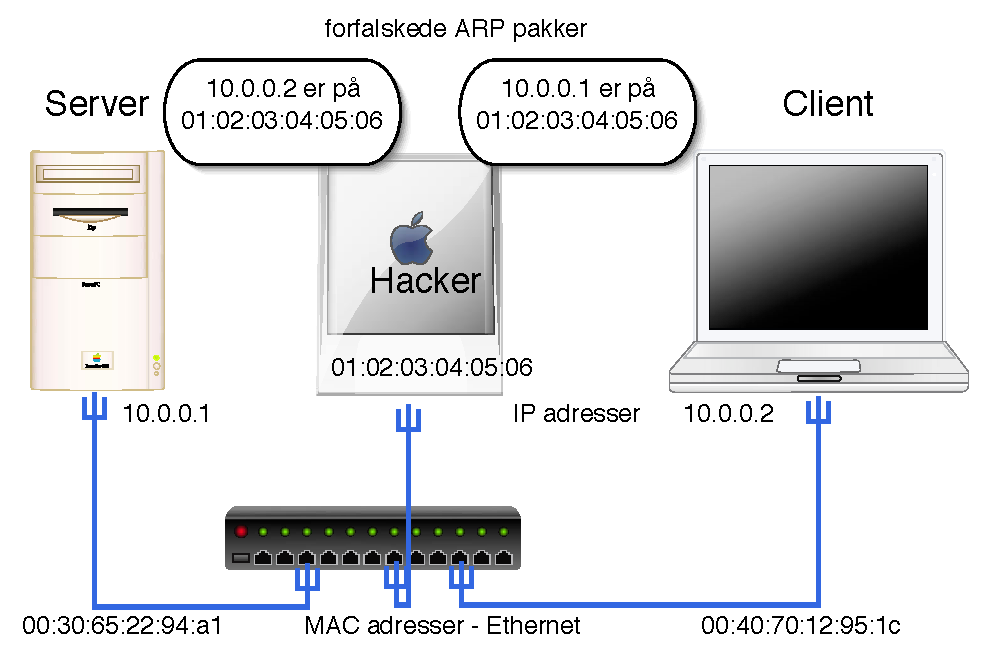
\includegraphics[width=12cm]{images/arp-spoof.pdf}}  
\end{center}

\begin{list1}
\item Afl�sning af hemmeligheder - kodeord m.v.
\item Hvilke foruds�tninger er der for at bruge Dsniff?
\item dsniff skal have adgang til trafikken ...
%\item P� et system med dsniff installeret findes manual siderne
%  {\bfseries man arpspoof} og {\bfseries man dsniff}
\end{list1}


%%% Local Variables: 
%%% mode: latex
%%% TeX-master: "tcpip-security"
%%% End: 


\slide{POP3 i Danmark}

\hlkimage{17cm}{images/pop3-1.pdf}

\begin{list1}
\item Man har tillid til sin ISP - der administrerer såvel net som server
\end{list1}

\slide{POP3 i Danmark - trådløst}

\hlkimage{14cm}{images/pop3-wlan.pdf}
\begin{list1}
\item Har man tillid til andre ISP'er? Alle ISP'er?
\item Deler man et netværksmedium med andre?
\end{list1}



\slide{POP3 netværk, demo}
%\slide{HTTP basic}

\hlkimage{16cm}{dsniff-passwords.png}

\centerline{Dsniff screenshot, vi viser måske Ethereal}

\slide{WEP kryptering}

%\begin{center}
%\colorbox{white}{
\includegraphics[width=12cm]{images/airsnort.pdf}}
%\end{center}
\begin{list1}
\item WEP \emph{kryptering} - med nøgler der specificeres som tekst
  eller hexadecimale cifre
\item typisk 40-bit, svarende til 5 ASCII tegn eller 10 hexadecimale
  cifre eller 104-bit 13 ASCII tegn eller 26 hexadecimale cifre
\item WEP er baseret på RC4 algoritmen der er en \emph{stream cipher}
  lavet af Ron Rivest for RSA Data Security
\end{list1}


\slide{De første fejl ved WEP}
\begin{list1}
\item Oprindeligt en dårlig implementation i mange Access Points
\item Fejl i krypteringen - rettet i nyere firmware
\item WEP er baseret på en DELT hemmelighed som alle stationer kender
\item Nøglen ændres sjældent, og det er svært at distribuere en ny
\end{list1}

\slide{WEP som sikkerhed}

\hlkimage{6cm}{images/no-wep.pdf}
\begin{list1}
\item WEP er \emph{ok} til et privat hjemmenetværk
\item WEP er for simpel til et større netværk - eksempelvis 20 brugere
\item Firmaer bør efter min mening bruge andre
  sikkerhedsforanstaltninger
\item Hvordan udelukker man en bestemt bruger?
\end{list1}


\slide{Cryptography}


\begin{list1}
\item Cryptography or cryptology is the practice and study of techniques for secure communication
\item Modern cryptography is heavily based on mathematical theory and computer science practice; cryptographic algorithms are designed around computational hardness assumptions, making such algorithms hard to break in practice by any adversary
\item Symmetric-key cryptography refers to encryption methods in which both the sender and receiver share the same key, to ensure confidentiality, example algorithm AES
\item Public-key cryptography (like RSA) uses two related keys, a key pair of a public key and a private key. This allows for easier key exchanges, and can provide confidentiality, and methods for signatures and other services
\end{list1}

Source: \link{https://en.wikipedia.org/wiki/Cryptography}

\slide{Kryptografiske principper}

\begin{list1}
\item Algoritmerne er kendte
\item Nøglerne er hemmelige
\item Nøgler har en vis levetid - de skal skiftes ofte
\item Et successfuldt angreb på en krypto-algoritme er enhver genvej
  som kræver mindre arbejde end en gennemgang af alle nøglerne
\item Nye algoritmer, programmer, protokoller m.v. skal gennemgås nøje!
\item Se evt. Snake Oil Warning Signs:
Encryption Software to Avoid\\
\link{http://www.interhack.net/people/cmcurtin/snake-oil-faq.html}
\end{list1}

\slide{DES, Triple DES og AES}

\hlkimage{15cm}{images/AES_head.png}

\begin{list1}
\item DES kryptering baseret på den IBM udviklede Lucifer algoritme
  har været benyttet gennem mange år
\item Der blev i 2001 vedtaget en ny standard algoritme Advanced Encryption
  Standard (AES) som afløser Data Encryption Standard (DES)
\item Algoritmen hedder Rijndael og er udviklet
af Joan Daemen og Vincent Rijmen.
%\item \emph{Rijndael is available for free. You can use it for
%whatever purposes  you want, irrespective of whether
%it is accepted as AES or not.}
\item Se også \link{https://en.wikipedia.org/wiki/Advanced_Encryption_Standard}
\end{list1}


\slide{Formålet med kryptering}

\vskip 3 cm
\centerline{\hlkbig kryptering er den eneste måde at sikre:}
\vskip 3 cm
\centerline{\hlkbig fortrolighed}
\vskip 3 cm
\centerline{\hlkbig autenticitet / integritet}


%%% Local Variables:
%%% mode: latex
%%% TeX-master: "tcpip-security"
%%% End:


\slide{WEP sikkerhed}

\hlkimage{12cm}{images/airsnort.pdf}

\begin{quote}
AirSnort is a wireless LAN (WLAN) tool which recovers encryption
keys. AirSnort operates by passively monitoring transmissions,
computing the encryption key when enough packets have been gathered.

802.11b, using the Wired Equivalent Protocol (WEP), is crippled with
numerous security flaws. Most damning of these is the weakness
described in " Weaknesses in the Key Scheduling Algorithm of RC4 "
by Scott Fluhrer, Itsik Mantin and Adi Shamir. Adam Stubblefield
was the first to implement this attack, but he has not made his
software public. AirSnort, along with WEPCrack, which was released
about the same time as AirSnort, are the first publicly available
implementaions of this attack.  \link{http://airsnort.shmoo.com/}
\end{quote}

%\begin{list1}
%\item i dag er firmware opdateret hos de fleste producenter
%\item men sikkerheden baseres stadig på een delt hemmelighed
%\end{list1}

\slide{major cryptographic errors}

\begin{list1}
\item weak keying - 24 bit er allerede kendt - 128-bit = 104 bit i praksis
\item small IV - med kun 24 bit vil hver IV blive genbrugt oftere
\item CRC-32 som intergritetscheck er ikke \emph{stærkt} nok
  kryptografisk set
\item Authentication gives pad - giver fuld adgang - hvis der bare
  opdages \emph{encryption pad} for en bestemt IV. Denne IV kan så
  bruges til al fremtidig kommunikation
\end{list1}
Source:
\emph{Secure Coding: Principles and Practices}, Mark G. Graff
  og Kenneth R. van Wyk, O'Reilly, 2003

\slide{Konklusion: Kryptografi er svært}

%Stoler vi på de andre autentificeringsmetoder?}
\hlkimage{20cm}{crypto-class.png}

Åbent kursus på Stanford\\
\link{http://crypto-class.org/}



\slide{WEP cracking - airodump og aircrack}

\hlkimage{3cm}{images/no-wep.pdf}

\begin{list1}
\item airodump - opsamling af krypterede pakker
\item aircrack - statistisk analyse og forsøg på at finde WEP nøglen
\item Med disse værktøjer er det muligt at knække \emph{128-bit nøgler}!
\item Blandt andet fordi det reelt er 104-bit nøgler \smiley
\item tommelfingerregel - der skal opsamles mange pakker ca. 500.000
  er godt, og ofte kan der knækkes med lang færre
\item Links:\\
\link{http://www.cr0.net:8040/code/network/aircrack/} aircrack\\
\link{http://www.securityfocus.com/infocus/1814} WEP: Dead Again
\end{list1}

\slide{airodump afvikling}

\begin{list1}
\item Når airodump kører opsamles pakkerne
\item samtidig vises antal initialisationsvektorer IV's:
\end{list1}

\vskip 1 cm

\begin{alltt}
\hlktiny
   BSSID              CH  MB  ENC  PWR  Packets   LAN IP / # IVs   ESSID

   00:03:93:ED:DD:8D   6  11       209   {\bf 801963                  540180}   wanlan
\end{alltt}

\vskip 2 cm

\begin{list1}
\item NB: dataopsamlingen er foretaget på 100\% opdateret Mac udstyr
\end{list1}


\slide{aircrack - WEP cracker}

\begin{alltt}
\footnotesize
   $ aircrack -n 128 -f 2 aftendump-128.cap
                                 aircrack 2.1
   * Got  540196! unique IVs | fudge factor = 2
   * Elapsed time [00:00:22] | tried 12 keys at 32 k/m
   KB    depth   votes
    0    0/  1   CE(  45) A1(  20) 7E(  15) 98(  15) 72(  12) 82(  12)
    1    0/  2   62(  43) 1D(  24) 29(  15) 67(  13) 94(  13) F7(  13)
    2    0/  1   B6( 499) E7(  18) 8F(  15) 14(  13) 1D(  12) E5(  10)
    3    0/  1   4E( 157) EE(  40) 29(  39) 15(  30) 7D(  28) 61(  20)
    4    0/  1   93( 136) B1(  28) 0C(  15) 28(  15) 76(  15) D6(  15)
    5    0/  2   E1(  75) CC(  45) 39(  31) 3B(  30) 4F(  16) 49(  13)
    6    0/  2   3B(  65) 51(  42) 2D(  24) 14(  21) 5E(  15) FC(  15)
    7    0/  2   6A( 144) 0C(  96) CF(  34) 14(  33) 16(  33) 18(  27)
    8    0/  1   3A( 152) 73(  41) 97(  35) 57(  28) 5A(  27) 9D(  27)
    9    0/  1   F1(  93) 2D(  45) 51(  29) 57(  27) 59(  27) 16(  26)
   10    2/  3   5B(  40) 53(  30) 59(  24) 2D(  15) 67(  15) 71(  12)
   11    0/  2   F5(  53) C6(  51) F0(  21) FB(  21) 17(  15) 77(  15)
   12    0/  2   E6(  88) F7(  81) D3(  36) E2(  32) E1(  29) D8(  27)
         {\color{red}\bf KEY FOUND! [ CE62B64E93E13B6A3AF15BF5E6 ]}
\end{alltt}
%$


\slide{Hvor lang tid tager det?}

\begin{list1}
\item Opsamling a data - ca. en halv time på 802.11b ved optimale forhold
\item Tiden for kørsel af aircrack fra auditor CD
på en Dell CPi 366MHz Pentium II laptop:
\end{list1}
\begin{alltt}

   $ time aircrack -n 128 -f 2 aftendump-128.cap
   ...
   real    5m44.180s   user  0m5.902s     sys  1m42.745s
   \end{alltt}
   %$

\pause
\begin{list1}
\item Tiden for kørsel af aircrack på en VIA CL-10000 1GHz CPU med
  almindelig disk OpenBSD:
\end{list1}
\begin{alltt}
   25.12s real     0.63s user     2.14s system
\end{alltt}

\slide{Erstatning for WEP - WPA}

\begin{list1}
\item Det anbefales at bruge:
%\begin{list2}
\item Kendte VPN teknologier eller WPA
\item baseret på troværdige algoritmer
\item implementeret i professionelt udstyr
\item fra troværdige leverandører
\item udstyr der vedligeholdes og opdateres
%\end{list2}
\item Man kan måske endda bruge de eksisterende løsninger - fra
  hjemmepc adgang, mobil adgang m.v.
\end{list1}


\slide{RADIUS}
\begin{list1}
\item RADIUS er en protokol til autentificering af brugere op mod en
  fælles server
\item Remote Authentication Dial In User Service (RADIUS)
\item RADIUS er beskrevet i RFC-2865
\item RADIUS kan være en fordel i større netværk med
\begin{list2}
\item dial-in
\item administration af netværksudstyr
\item trådløse netværk
\item andre RADIUS kompatible applikationer
\end{list2}
\end{list1}

\slide{Erstatninger for WEP}
\begin{list1}
\item Der findes idag andre metoder til sikring af trådløse netværk
\item 802.1x Port Based Network Access Control
\item WPA - Wi-Fi Protected Access)\\
WPA = 802.1X + EAP + TKIP + MIC
\item nu WPA2
\begin{quote}
WPA2 is based on the final IEEE 802.11i amendment to the 802.11
standard and is eligible for FIPS 140-2 compliance.
\end{quote}
\item Source:
\href{http://www.wifialliance.org/OpenSection/protected_access.asp}
{http://www.wifialliance.org/OpenSection/protected\_access.asp}
\end{list1}


\slide{WPA eller WPA2?}

\begin{quote}
WPA2 is based upon the Institute for Electrical and Electronics
Engineers (IEEE) 802.11i amendment to the 802.11 standard, which was
ratified on July 29, 2004.
\end{quote}

\begin{quote}
Q: How are WPA and WPA2 similar?\\
A: Both WPA and WPA2 offer a high level of assurance for end-users and network
administrators that their data will remain private and access to their
network restricted to authorized users.
Both utilize 802.1X and Extensible Authentication Protocol (EAP) for
authentication. Both have Personal and Enterprise modes of operation
that meet the distinct needs of the two different consumer and
enterprise market segments.

Q: How are WPA and WPA2 different?\\
A: WPA2 provides a {\bf stronger encryption mechanism} through {\bf
  Advanced Encryption Standard (AES)}, which is a requirement for some
corporate and government users.
\end{quote}

\centerline{Source: http://www.wifialliance.org WPA2 Q and A}

\slide{WPA Personal eller Enterprise}

\begin{list1}
\item Personal - en delt hemmelighed, preshared key
\item Enterprise - brugere valideres op mod fælles server
\item Hvorfor er det bedre?
\begin{list2}
\item Flere valgmuligheder - passer til store og små
\item WPA skifter den faktiske krypteringsnøgle jævnligt - TKIP
\item Initialisationsvektoren (IV) fordobles 24 til 48 bit
\item Imødekommer alle kendte problemer med WEP!
\item Integrerer godt med andre teknologier - RADIUS

\vskip 1 cm
\item EAP - Extensible Authentication Protocol - individuel autentifikation
\item TKIP - Temporal Key Integrity Protocol - nøgleskift og integritet
\item MIC - Message Integrity Code - Michael, ny algoritme til integritet
\end{list2}

\end{list1}


\slide{WPA cracking}

\begin{list1}
\item Nu skifter vi så til WPA og alt er vel så godt?
\pause
\item Desværre ikke!
\item Du skal vælge en laaaaang passphrase, ellers kan man sniffe WPA
  handshake når en computer går ind på netværket!
\item Med et handshake kan man med aircrack igen lave off-line
  bruteforce angreb!
\end{list1}

\slide{WPA cracking demo}

\begin{list1}
\item Vi konfigurerer AP med Henrik42 som WPA-PSK/passhrase
\item Vi finder netværk kismet eller airodump
\item Vi starter airodump mod specifik kanal
\item Vi spoofer deauth og opsamler WPA handshake
\item Vi knækker WPA :-)
\end{list1}

\centerline{Brug manualsiderne for programmerne i aircrack-ng pakken!}

\slide{WPA cracking med aircrack - start}

\begin{alltt}
\small
slax ~ # aircrack-ng -w dict wlan-test.cap
Opening wlan-test.cap
Read 1082 packets.

#  BSSID              ESSID           Encryption

1  00:11:24:0C:DF:97  wlan            WPA (1 handshake)
2  00:13:5F:26:68:D0  Noea            No data - WEP or WPA
3  00:13:5F:26:64:80  Noea            No data - WEP or WPA
4  00:00:00:00:00:00                  Unknown

Index number of target network ? {\bf 1}
\end{alltt}

\slide{WPA cracking med aircrack - start}

\begin{alltt}
\small
          [00:00:00] 0 keys tested (0.00 k/s)

                    KEY FOUND! [ Henrik42 ]

Master Key     : 8E 61 AB A2 C5 25 4D 3F 4B 33 E6 AD 2D 55 6F 76
                 6E 88 AC DA EF A3 DE 30 AF D8 99 DB F5 8F 4D BD
Transcient Key : C5 BB 27 DE EA 34 8F E4 81 E7 AA 52 C7 B4 F4 56
                 F2 FC 30 B4 66 99 26 35 08 52 98 26 AE 49 5E D7
                 9F 28 98 AF 02 CA 29 8A 53 11 EB 24 0C B0 1A 0D
                 64 75 72 BF 8D AA 17 8B 9D 94 A9 31 DC FB 0C ED

EAPOL HMAC     : 27 4E 6D 90 55 8F 0C EB E1 AE C8 93 E6 AC A5 1F

\end{alltt}

\vskip 1 cm

\centerline{Min Thinkpad X31 med 1.6GHz Pentium M knækker ca. 150 Keys/sekund}

\centerline{Men hvem bruger en 1.6GHz Pentium M idag \smiley}

\slide{Encryption key length}

\hlkimage{19cm}{encryption-crack.png}

Source: \link{http://www.mycrypto.net/encryption/encryption_crack.html}

\slide{WPA cracking med Pyrit}

\begin{quote}
\emph{Pyrit} takes a step ahead in attacking WPA-PSK and WPA2-PSK, the protocol that today de-facto protects public WIFI-airspace. The project's goal is to estimate the real-world security provided by these protocols. Pyrit does not provide binary files or wordlists and does not encourage anyone to participate or engage in any harmful activity. {\bf This is a research project, not a cracking tool.}

\emph{Pyrit's} implementation allows to create massive databases, pre-computing part of the WPA/WPA2-PSK authentication phase in a space-time-tradeoff. The performance gain for real-world-attacks is in the range of three orders of magnitude which urges for re-consideration of the protocol's security. Exploiting the computational power of GPUs, \emph{Pyrit} is currently by far the most powerful attack against one of the world's most used security-protocols.
\end{quote}

\begin{list1}
%\item sloooow, plejede det at være -  ca 150 keys/s på min Thinkpad X31
\item Kryptering afhænger af SSID - så skift altid SSID!
\item \link{http://pyrit.wordpress.com/about/}
\end{list1}

\slide{Tired of WoW?}

\hlkimage{22cm}{pyritperfaa3.png}

Source: \link{http://code.google.com/p/pyrit/} Note old data!

\slide{Hashcat Cracking passwords and secrets}

\begin{list2}
\item Hashcat is the world's fastest CPU-based password recovery tool.
\item oclHashcat-plus is a GPGPU-based multi-hash cracker using a brute-force attack (implemented as mask attack), combinator attack, dictionary attack, hybrid attack, mask attack, and rule-based attack.
\item oclHashcat-lite is a GPGPU cracker that is optimized for cracking performance. Therefore, it is limited to only doing single-hash cracking using Markov attack, Brute-Force attack and Mask attack.
\item John the Ripper password cracker old skool men stadig nyttig
\end{list2}

Source:\\
\link{http://hashcat.net/wiki/}\\
\link{http://www.openwall.com/john/}\\
\link{http://hashcat.net/wiki/doku.php?id=cracking_wpawpa2}



\slide{ Wi-Fi Protected Setup, WPS hacking - Reaver}

\begin{quote}
Reaver Open Source
Reaver implements a brute force attack against Wifi Protected Setup (WPS) registrar PINs in order to recover WPA/WPA2 passphrases, as described in \link{http://sviehb.files.wordpress.com/2011/12/viehboeck_wps.pdf}.

Reaver has been designed to be a robust and practical attack against WPS, and has been tested against a wide variety of access points and WPS implementations.

On average Reaver will recover the target AP's plain text WPA/WPA2 passphrase in 4-10 hours, depending on the AP. In practice, it will generally take half this time to guess the correct WPS pin and recover the passphrase.
\end{quote}

\centerline{Hvad betyder ease of use?}

Source: \\
\link{https://code.google.com/p/reaver-wps/}\\
{\footnotesize \link{http://lifehacker.com/5873407/how-to-crack-a-wi+fi-networks-wpa-password-with-reaver}}

\slide{WPS Design Flaws used by Reaver }

\hlkimage{22cm}{wps-design-flaw-1.png}

\centerline{Pin only, no other means necessary}

Source:\\
\link{http://sviehb.files.wordpress.com/2011/12/viehboeck_wps.pdf}



\slide{WPS Design Flaws used by Reaver }

\hlkimage{14cm}{wps-design-flaw-2.png}

\centerline{Reminds me of NTLM cracking, crack parts independently}

Source:\\
\link{http://sviehb.files.wordpress.com/2011/12/viehboeck_wps.pdf}



\slide{WPS Design Flaws used by Reaver }

\hlkimage{23cm}{wps-design-flaw-2-2.png}

\centerline{100.000.000 is a lot, 11.000 is not}

Source:\\
\link{http://sviehb.files.wordpress.com/2011/12/viehboeck_wps.pdf}






\slide{Reaver Rate limiting}

\hlkimage{18cm}{reaver-rate-limiting.png}


\slide{Opsummering}

\begin{list1}
\item De fleste trådløse enheder leveres med en standard
  konfiguration som er helt åben!
\item det første man kan gøre er at slå noget kryptering til
\item Brug ikke WEP men \emph{noget andet} - WPA, Cisco LEAP, VPN,
  IPsec, ...
\item Derudover kan en del access points filtrere på MAC adresser glem
  det
\item på visse AP er der mulighed for opslag på RADIUS servere -
  Remote Authentication Dial In User Service (RADIUS)
\end{list1}




\slide{wireless specifikke hacks}

\begin{center}
\colorbox{white}{
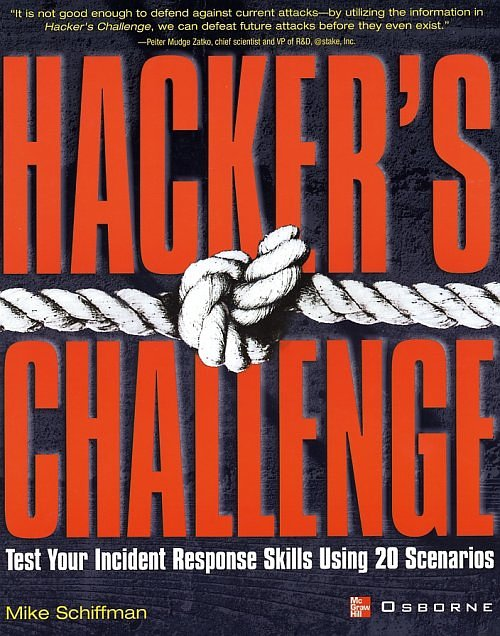
\includegraphics[width=33mm]{images/hackers-challenge.jpg}
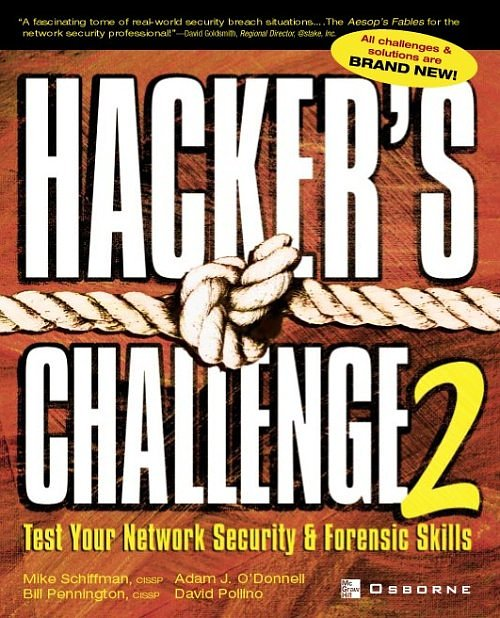
\includegraphics[width=33mm]{images/hackers-challenge2.jpg}}
\end{center}

\begin{list1}
\item Hackers Challenge 2 - disassociate attack
\item OpenBSD program - fremprovokere traffik så der kan knækkes WEP
findes på Packetstorm med navnet wnet.tgz lavet til OpenBSD 3.2
% Included in this base package are dinject v0.1, a command line
% 802.11b packet injection package based on nemesis, and reinj v0.1, a
% proof-of-concept utility for the tcp/arp re-injection attack to
% generate traffic on a weped network. This tool will allow an
% end-user to crack WEP on a low-traffic network in less than 60
% minutes. It is for OPENBSD 3.2 only.
\end{list1}

\begin{center}
\small \emph{Hacker's Challenge : Test Your Incident Response Skills
    Using 20 Scenarios} af Mike Schiffman

\emph{Hacker's Challenge II : Test Your Network Security and Forensics
  Skills} af Mike Schiffman
\end{center}


% check også lige
% otto:~/projects/security/wireless/bellardo hlk$ pwd
% /Users/hlk/projects/security/wireless/bellardo


% otto:~/projects/security/wireless hlk$ open wlan_probemonitor.pdf
% otto:~/projects/security/wireless hlk$ pwd
% /Users/hlk/projects/security/wireless

\slide{Normal WLAN brug}

\hlkimage{20cm}{images/wlan-airpwn-1.pdf}

\slide{Packet injection - airpwn}

\hlkimage{20cm}{images/wlan-airpwn-2.pdf}

\slide{Airpwn teknikker}

\begin{list1}
\item Klienten sender forespørgsel
\item Hackerens program airpwn lytter og sender så falske pakker
\item Hvordan kan det lade sig gøre?
\begin{list2}
\item Normal forespørgsel og svar på Internet tager 50ms
\item Airpwn kan svare på omkring 1ms angives det
\item Airpwn har alle informationer til rådighed
\end{list2}
\item Airpwn på Defcon 2004 - findes på Sourceforge\\
\link{http://airpwn.sourceforge.net/}
\item NB: Airpwn som demonstreret er begrænset til TCP og ukrypterede
  forbindelser
\end{list1}



\slide{Når adgangen er skabt}

\begin{list1}
\item Så går man igang med de almindelige værktøjer
\item SecTools.Org: Top 125 Network Security Tools \link{http://www.sectools.org}
\end{list1}
\vskip 2 cm

\centerline{\hlkbig Forsvaret er som altid - flere lag af sikkerhed! }

\slide{Infrastrukturændringer}

\begin{center}
\colorbox{white}{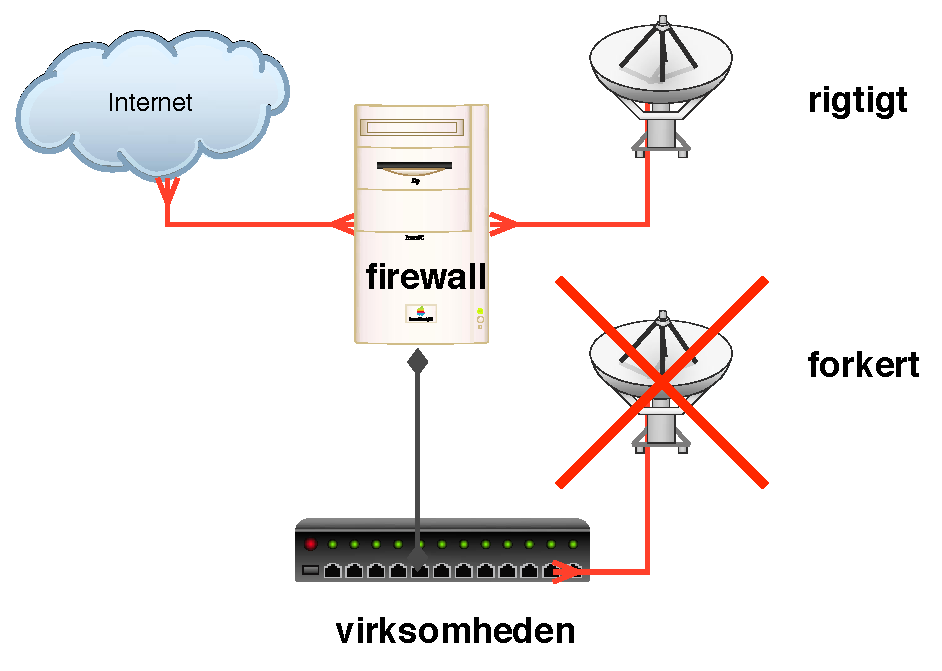
\includegraphics[height=11cm]{images/wlan-accesspoint-2.pdf}}
\end{center}

\centerline{\hlkbig Sådan bør et access point forbindes til netværket}




\slide{VLAN Virtual LAN}

\hlkimage{10cm}{vlan-portbased.pdf}

\begin{list2}
\item Nogle switche tillader at man opdeler portene
\item Denne opdeling kaldes VLAN og portbaseret er det mest simple
\item Port 1-4 er et LAN
\item De resterende er et andet LAN
\item Data skal omkring en firewall eller en router for at krydse fra VLAN1 til VLAN2
\end{list2}

\slide{IEEE 802.1q}

\hlkimage{18cm}{vlan-8021q.pdf}

\begin{list2}
\item Nogle switche tillader at man opdeler portene, men tillige benytter 802.1q
\item Med 802.1q tillades VLAN tagging på Ethernet niveau
\item Data skal omkring en firewall eller en router for at krydse fra VLAN1 til VLAN2
\item VLAN trunking giver mulighed for at dele VLANs ud på flere switches
\item Der findes administrationsværktøjer der letter dette arbejde: OpenNAC FreeNAC, Cisco VMPS
\end{list2}



\slide{Anbefalinger mht. trådløse netværk}

\begin{minipage}{10cm}
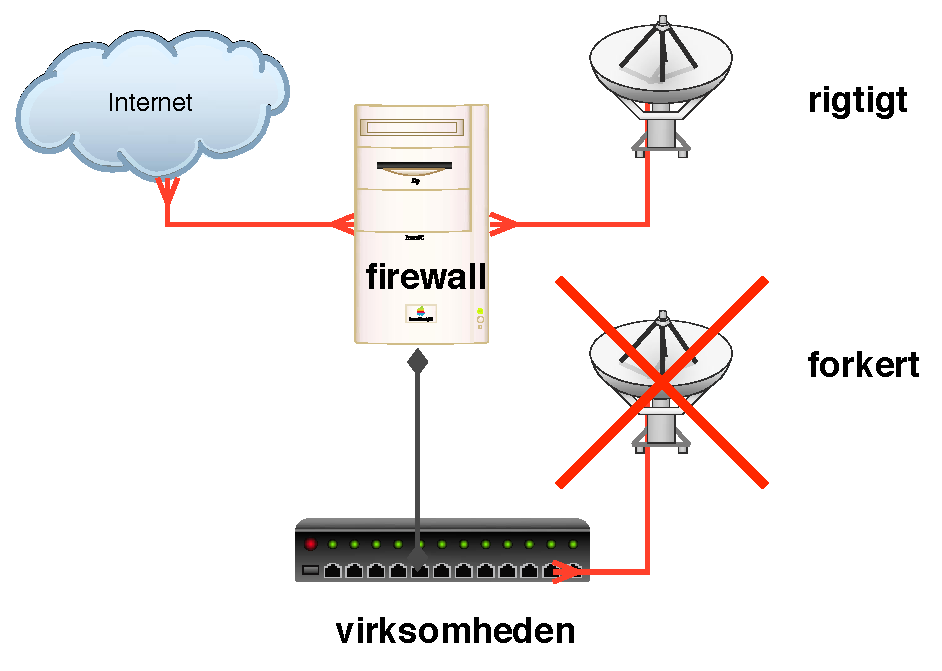
\includegraphics[width=10cm]{images/wlan-accesspoint-2.pdf}
\end{minipage}
\begin{minipage}{\linewidth-10cm}
\begin{list2}
\item Brug noget tilfældigt som SSID - netnavnet
\item Brug ikke WEP til virksomhedens netværk\\
- men istedet en VPN løsning med individuel
  autentificering eller WPA
\item NB: WPA Personal/PSK kræver passphrase på mange tegn! +40?
\item Placer de trådløse adgangspunkter hensigtsmæssigt i netværket -
  så de kan overvåges
\item Lav et sæt regler for brugen af trådløse netværk - hvor må
  medarbejdere bruge det?
\item Se eventuelt pjecerne \emph{Beskyt dit trådløse Netværk} fra
Ministeriet for Videnskab, Teknologi og Udvikling \\
\link{http://www.videnskabsministeriet.dk/}
\end{list2}
\end{minipage}


\slide{Hjemmenetværk for nørder}

\begin{list1}
\item Lad være med at bruge et wireless-kort i en PC til at lave AP, brug et AP
\item Husk et AP kan være en router, men den kan ofte også blot være en bro
\item Brug WPA og overvej at lave en decideret DMZ til WLAN
\item Placer AP hensigtsmæddigt og gerne højt, oppe på et skab eller lignende
\end{list1}



\slide{IEEE 802.1x  Port Based Network Access Control}

\hlkimage{12cm}{osx-8021x.png}

\begin{list2}
\item Nogle switche tillader at man benytter 802.1x
\item Denne protokol sikrer at man valideres før der gives adgang til porten
\item Når systemet skal have adgang til porten afleveres brugernavn og kodeord/certifikat
\item Denne protokol indgår også i WPA Enterprise
\end{list2}


\slide{802.1x og andre teknologier}

\begin{list1}
\item 802.1x i forhold til MAC filtrering giver væsentlige fordele
\item MAC filtrering kan spoofes, hvor 802.1x kræver det rigtige kodeord
\item Typisk benyttes RADIUS og 802.1x integrerer således mod både LDAP og Active Directory
\end{list1}




\slide{Undgå standard indstillinger}

\begin{list1}
\item når vi scanner efter services går det nemt med at finde dem
\item Giv jer selv mere tid til at omkonfigurere og opdatere ved at undgå standardindstillinger
\item Tiden der går fra en sårbarhed annonceres til den
  bliver udnyttet er meget kort idag!
\item Ved at undgå standard indstillinger kan der
  måske opnås en lidt længere frist - inden ormene kommer
\item NB: ingen garanti - og det hjælper sjældent mod en dedikeret angriber
\end{list1}


\slide{Next step, software sikkerhed}

\hlkimage{18cm}{software.pdf}

\centerline{Wireless AP implementerer protokoller med hardware+software}

\slide{Sårbare AP'er - 1}
\begin{list1}
\item Hvordan bygger man et billigt Access Point?
\begin{list2}
\item En embedded kerne
\item En embedded TCP/IP stak
\item Noget 802.11 hardware
\item Et par Ethernet stik
\item eventuelt et modem
\item Tape ...
\end{list2}
\item Hvad med efterfølgende opdatering af software?
\end{list1}

\slide{Sårbare AP'er - 2}
\begin{list1}
\item Eksempler på access point sårbarheder:
\item Konfigurationsfilen kan hentes uden autentificering - inkl. WEP
  nøgler
\item Konfigurationen sker via SNMP - som sender community string i
  klar tekst
\item  Wi-Fi Protected Setup,(WPS) kan ikke slås helt fra
\item ...
\item Konklusionen er klar - hardwaren er i mange tilfælde ikke sikker
  nok til at anvende på forretningskritiske LAN segmenter!
\end{list1}


\slide{Hvordan finder man buffer overflow, og andre fejl}

\begin{list1}
\item Black box testing
\item Closed source reverse engineering
\item White box testing
\item Open source betyder man kan læse og analysere koden
\item Source code review - automatisk eller manuelt
\item Fejl kan findes ved at prøve sig frem - fuzzing
\item Exploits virker typisk mod specifikke versioner af software
\end{list1}
\slide{Forudsætninger}

\begin{list1}
\item Bemærk: alle angreb har forudsætninger for at virke
\item Et angreb mod Telnet virker kun hvis du bruger Telnet
\item Et angreb mod Apache HTTPD virker ikke mod Microsoft IIS
\item Kan du bryde kæden af forudsætninger har du vundet!
\end{list1}


\slide{buffer overflows et C problem}

\begin{list1}
\item {\bfseries Et buffer overflow}
er det der sker når man skriver flere data end der er afsat plads til
i en buffer, et dataområde. Typisk vil programmet gå ned, men i visse
tilfælde kan en angriber overskrive returadresser for funktionskald og
overtage kontrollen.
\item {\bfseries Stack protection}
er et udtryk for de systemer der ved hjælp af operativsystemer,
programbiblioteker og lign. beskytter stakken med returadresser og
andre variable mod overskrivning gennem buffer overflows. StackGuard
og Propolice er nogle af de mest kendte.
\end{list1}


\slide{Buffer og stacks}

\hlkimage{20cm}{buffer-overflow-1.pdf}

\begin{alltt}
main(int argc, char **argv)
\{      char buf[200];
        strcpy(buf, argv[1]);
        printf("%s\textbackslash{}n",buf);
\}
\end{alltt}


\slide{Overflow - segmentation fault }

\hlkimage{20cm}{buffer-overflow-2.pdf}


\begin{list1}
\item Bad function overwrites return value!
\item Control return address
\item Run shellcode from buffer, or from other place
\end{list1}


\slide{Exploits - udnyttelse af sårbarheder}

\begin{list1}
\item exploit/exploitprogram er
\begin{list2}
\item udnytter eller demonstrerer en sårbarhed
\item rettet mod et specifikt system.
\item kan være 5 linier eller flere sider
\item Meget ofte Perl eller et C program
\end{list2}
\end{list1}


\slide{Exploits}

\vskip 1 cm

\begin{alltt}
$buffer = "";
$null = "\textbackslash{}x00"; \pause
$nop = "\textbackslash{}x90";
$nopsize = 1; \pause
$len = 201; // what is needed to overflow, maybe 201, maybe more!
$the_shell_pointer = 0xdeadbeef; // address where shellcode is
# Fill buffer
for ($i = 1; $i < $len;$i += $nopsize) \{
    $buffer .= $nop;
\}\pause
$address = pack('l', $the_shell_pointer);
$buffer .= $address;\pause
exec "$program", "$buffer";
\end{alltt}
\vskip 1 cm
\centerline{Demo exploit in Perl}
%Eksempel på webserver buffer overflow, nosejob?

\slide{Wireless buffer overflows beware of the {\bf BLOB}}

\hlkimage{8cm}{Blob.jpg}

\centerline{AP and driver software has errors, some exploitable}


% too old
%\slide{Black Hat Briefings 2006}

%\begin{list1}
%\item Black Hat Briefings 2006.
%\item Der er kommet diverse rettelser til Apple Mac OS X
%\item Apple wireless vulnerable after all\\
%\link{http://www.securityfocus.com/brief/311}
%\end{list1}

%\slide{Flere links}

%\begin{list1}
%\item Vi har måske ikke tid til mere, men fri snak og diskussion nu
%\item \link{http://kernelfun.blogspot.com/}
%\item \link{http://www.802.11mercenary.net/}
%\item \link{http://toorcon.org/2006/conference.html}
%\item Der sker meget indenfor wireless!
%\end{list1}


\slide{24 Deadly Sins of Software Security}

\hlkrightimage{5cm}{24-deadly.jpg}
\emph{24 Deadly Sins of Software Security} af Michael Howard, David Leblanc, John Viega 2009

\begin{list1}
\item {\bf Obligatorisk læsning for alle udviklere}
\item Denne bog er præcis og giver overblik på kun 432 sider
\item Buffer Overruns, Format String Problems, Integer Overflows, SQL Injection, Command Injection,
Failing to Handle Errors, Cross-Site Scripting, Failing to Protect Network Traffic, Magic URLs Hidden Form Fields,
Improper Use of SSL and TLS, Weak Password-Based Systems, Failing to Store and Protect Data Securely, Information
Leakage, Improper File Access, Trusting Network Name Resolution, Race Conditions, Unauthenticated Key Exchange, Cryptographically Strong Random Numbers, Poor Usability
\end{list1}






\slide{Recommendations for wireless networks}

\begin{minipage}{10cm}
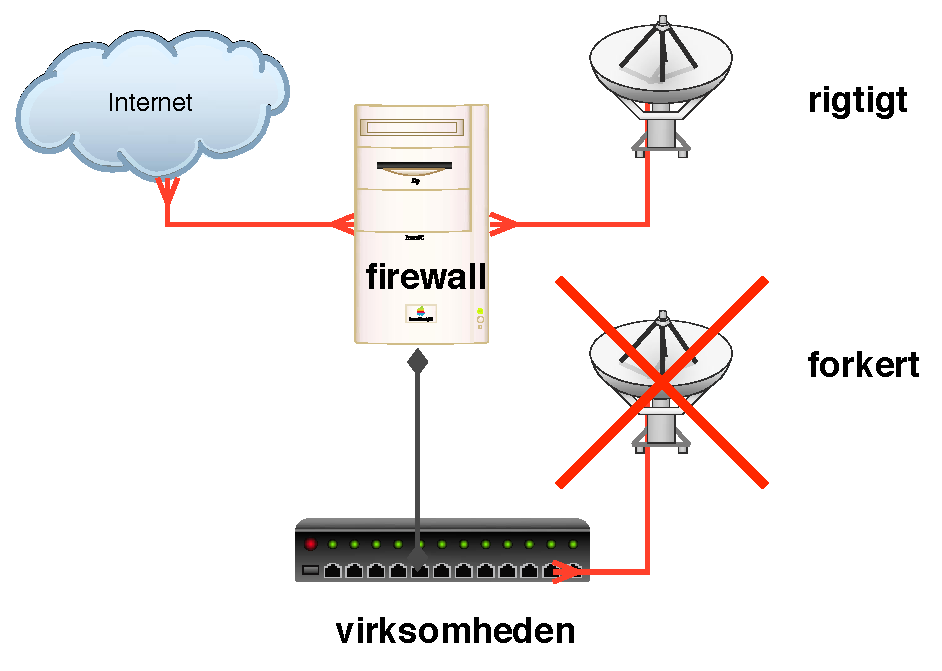
\includegraphics[width=10cm]{images/wlan-accesspoint-2.pdf}
\end{minipage}
\begin{minipage}{\linewidth-10cm}
\begin{list2}
\item Use a specific SSID - network name, influences the WPA PSK keying
\item Never use WEP
\item Use WPA PSK or Enterprise, or at least some VPN with individual user logins

\item When using WPA Personal/PSK passphrase must be long, like +40 chars!
\item Place network Access Points on the network where they can be monitored. Seperate VLAN, isolated from the cabled LAN
\item Have rules for the use of wireless networks, also for persons travelling - "Always use VPN when using insecure wireless in hotels, airports etc."
\end{list2}
\end{minipage}



\slide{Summary}

\begin{list1}
\item Husk følgende:
\begin{list2}
\item Husk: IT-sikkerhed er ikke kun netværkssikkerhed!
\item Sikkerhed kommer fra langsigtede intiativer\\
 {\bfseries Vi håber I kan genkende de problemer vi har talt om,
    og finde information om nye problemer i netværk som bliver kendt\\
 eksempelvis nye metoder til scanning eller omgåelse af
    firewalls}
\item Hvad er informationssikkerhed?
\item Data på elektronisk form
\item Data på fysisk form
\item Social engineering er måske overset - \emph{The Art of Deception:
Controlling the Human Element of Security}
af Kevin D. Mitnick, William L. Simon, Steve Wozniak
\end{list2}
\item Computer Forensics er reaktion på en hændelse
\item {\bfseries Informationssikkerhed er en proces}
\end{list1}




\myquestionspage


\slide{Hackers Challenge}

\begin{center}
\colorbox{white}{
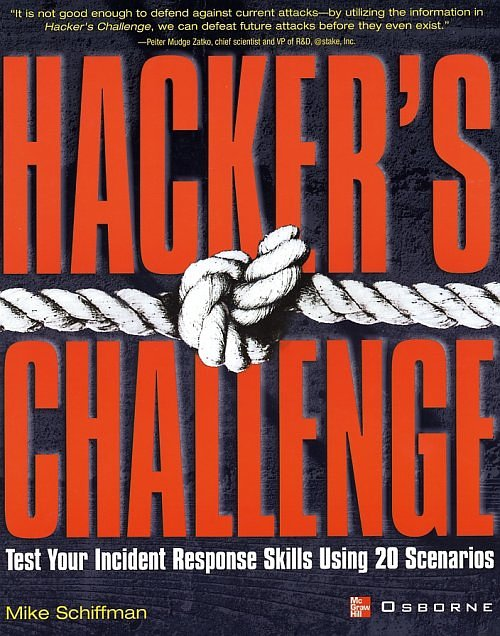
\includegraphics[width=32mm]{images/hackers-challenge.jpg}
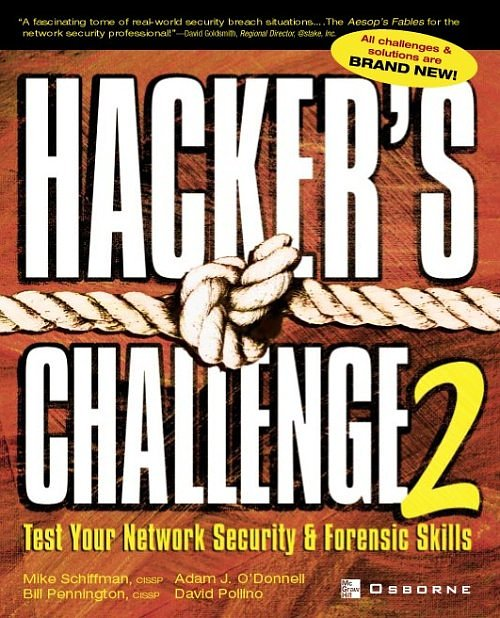
\includegraphics[width=33mm]{images/hackers-challenge2.jpg}
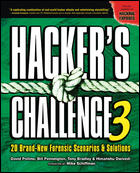
\includegraphics[width=33mm]{images/hackers-challenge-3.jpg}}
\end{center}

\begin{list1}
%\item Hændelseshåndtering - øvelse som I kigger på i weekenden
%\item Opgaverne er kopieret fra bogen
\item \emph{Hacker's Challenge: Test Your Incident Response Skills Using 20 Scenarios} McGraw-Hill Osborne Media; (October 18, 2001) ISBN:
 0072193840
\item \emph{Hacker's Challenge 2: Test Your Network Security and
 Forensics Skills} McGraw-Hill Osborne Media, 2003 ISBN: 0072226307
\item \emph{Hacker's Challenge 3: 20 Brand New Forensic Scenarios \& Solutions} McGraw-Hill Osborne Media; 3 edition (April 25, 2006) ISBN: 0072263040
\item These books contain scenarios and solutions. Focus on a few critical logs and then some questions to be answered from the data available.
\end{list1}

\end{document}
